\documentclass{article}
\PassOptionsToPackage{numbers, compress}{natbib}
\usepackage[dblblindworkshop]{neurips_2026}
\workshoptitle{New in Machine Learning (NewInML)}

\usepackage[utf8]{inputenc}
\usepackage[T1]{fontenc}
\usepackage{hyperref}
\usepackage{url}
\usepackage{booktabs}
\usepackage{amsfonts}
\usepackage{amsmath, amssymb}
\usepackage{nicefrac}
\usepackage{microtype}
\usepackage{xcolor}
\usepackage{multirow}
\usepackage{float}
\usepackage{tikz}
\usetikzlibrary{shapes.geometric, arrows.meta, positioning, fit, backgrounds}

\tikzset{
  mainbox/.style={rectangle, rounded corners=4pt, minimum width=8cm, minimum height=1.0cm,
    text centered, text width=7.8cm, font=\small\bfseries, inner sep=6pt},
  navybox/.style={mainbox, fill=blue!25!black, text=white},
  bluebox/.style={mainbox, fill=blue!55, text=white},
  lightbox/.style={mainbox, fill=blue!10, text=blue!30!black, draw=blue!40, line width=0.8pt},
  greenbox/.style={mainbox, fill=green!35!black, text=white},
  brownbox/.style={mainbox, fill=orange!40!brown, text=white},
  warmbox/.style={mainbox, fill=orange!15, text=orange!40!brown, draw=orange!40!brown, line width=0.8pt},
  purplebox/.style={mainbox, fill=violet!60!black, text=white},
  clusterbox/.style={rectangle, rounded corners=3pt, minimum width=2.3cm, minimum height=0.9cm,
    text centered, text width=2.1cm, font=\small\bfseries, fill=green!15, draw=green!40!black,
    line width=0.8pt, text=green!30!black},
  arrow/.style={-Stealth, thick, blue!40!black}
}

\title{Peer-Isolated Recommendation: When Content-Only Personalization Beats Collaborative Signal, and When It Doesn't\footnotemark}

\author{%
  Anonymous Author(s) \\
  Affiliation \\
  Address \\
  \texttt{email}
}

\begin{document}

\maketitle
\footnotetext{Code and data: \url{https://anonymous.4open.science/r/essence-5B7B/README.md}}

\begin{abstract}
We present Essence, a personal embedding cluster framework for recommendation that operates exclusively within a single user's engagement history, without consulting cross-user interaction data. We evaluate Essence on three datasets spanning distinct domains --- Last.fm-1K (music), Amazon Books (e-commerce), and MovieLens-25M (film) --- against a real collaborative-filtering baseline, a non-personalized popularity baseline, a content-based average-embedding baseline, three recency-based baselines (last-item, uniform-average, and exponentially-weighted retrieval), and two hand-implemented multi-interest neural baselines (MIND, ComiRec). Essence's performance relative to these baselines is domain-dependent, and the dependence has a specific, testable shape: Essence's rank among the ten evaluated systems tracks inversely with the strength of collaborative/popularity signal available in the domain. On Amazon Books, where collaborative and popularity baselines are structurally weak (Recall@10 of $0.0031$ and $0.0021$ respectively), Essence does not lead on Recall@10 among personalized methods --- three recency-based baselines score higher (Last-Item $0.0311$, Recency-Weighted $0.0260$, Avg-Last-10 $0.0235$, vs.\ Essence's $0.0221$), and Essence loses significantly to Last-Item and Recency-Weighted after FDR correction ($d=-0.090$, $d=-0.059$). Essence's Amazon strength is narrower: it significantly beats collaborative filtering, popularity, content-averaging, and both neural multi-interest baselines on Recall@10 ($d$ ranges $0.069$--$0.259$), and significantly beats Popularity, Random, Content, and MIND on LT-Recall@10 specifically; it is statistically tied with CF-ItemKNN, ComiRec, Last-Item, Recency-Weighted, and Avg-Last-10 on LT-Recall@10. On MovieLens-25M, where collaborative signal is strong (item-based CF reaches $0.0850$ Recall@10, driven almost entirely by the platform's densely-rated popular titles), Essence ranks 8th of 10 systems, losing to collaborative filtering, popularity, and both neural baselines by the largest effect sizes observed in this study (Cohen's $d$ up to $-0.56$). On Last.fm-1K, simple recency-based retrieval (no clustering) outperforms Essence outright. We report every comparison with paired bootstrap significance testing ($10{,}000$ resamples), Benjamini--Hochberg correction for multiple comparisons, standardized effect sizes, and BCa robustness cross-checks --- replacing an earlier confidence-interval-overlap methodology that does not test the quantity of interest. A targeted stratification test finds that $K$-means clustering, isolated from recency-weighted retrieval, provides no measurable benefit even for the users it is theoretically best suited to help: those with the most well-separated, multi-modal interest histories. We frame Essence not as a universally superior candidate generator, but as a data point on when peer-isolated, content-only personalization is and isn't the right architectural choice, and as a case study in what a fair, statistically grounded, honestly-reported evaluation of a recommendation architecture looks like when the result is mixed.
\end{abstract}

\section{Introduction}
\label{sec:intro}

Collaborative filtering (CF) predicts a user's future preferences from the behavior of similarly-behaving users. Items with sparse interaction histories are, by construction, underrepresented in any signal derived from cross-user co-occurrence: a user with a narrow, idiosyncratic taste profile receives recommendations shaped by aggregate similarity to other users, not by the specific combination of properties their own history reflects.

This motivates two questions. First: can a recommendation signal be constructed using only a single user's own history, without any cross-user data, and if so, does it recover items that collaborative methods structurally underrepresent? Second, answerable only once the same comparison is run across multiple, structurally different domains: under what domain conditions does this approach help versus hurt, and is the effect predictable from properties of the domain rather than discovered post hoc per dataset? A one- or two-dataset evaluation cannot distinguish a domain-general advantage from a domain-specific artifact; the three-dataset evaluation reported here is designed specifically to make that distinction possible.

We propose Essence, a framework that embeds a user's consumed items into a semantic space, clusters them into $K$ interest profiles via $K$-means, and generates recommendations by retrieving items similar to the centroid closest to the user's recent activity. No cross-user interaction graph is consulted at any stage (the \emph{peer-isolation property}) --- a deliberate architectural constraint, not an oversight.

Contributions: (1) the Essence architecture, requiring no collaborative signal and no cross-user training; (2) a recency-based active-cluster-selection mechanism, evaluated via ablation against a static mean-embedding alternative and against three recency-only baselines that do not cluster at all; (3) a domain-dependence finding across three datasets spanning music, e-commerce, and film, with effect sizes ranging from Essence's strongest win ($d=+0.259$, Amazon Books vs.\ Random) to its strongest loss ($d=-0.558$, MovieLens-25M vs.\ CF-ItemKNN); (4) two hand-implemented multi-interest neural baselines (MIND, ComiRec), verified against their architectural specifications rather than against published benchmark numbers (Section~\ref{sec:setup}), including a symmetry-breaking bug caught in our own MIND implementation --- not the original architecture --- by a synthetic conformance test before any number reported here was generated; and (5) a statistical-methodology correction (paired bootstrap, Benjamini--Hochberg FDR, effect sizes, BCa cross-checks) applied uniformly across all three datasets, replacing an earlier confidence-interval-overlap methodology.

\section{Related Work}
\label{sec:related}

\textbf{Collaborative filtering.} Matrix factorisation~\cite{koren2009} and neural extensions~\cite{he2017} remain dominant in production recommendation, but are optimised for the median user: they perform well on what is broadly consumed and comparatively weakly on what is individually resonant.

\textbf{Multi-interest retrieval.} MIND~\cite{li2019} introduced dynamic routing to extract multiple interest capsules from a user's history; ComiRec~\cite{cen2020} extended this with explicit diversity controls. Essence shares the multi-interest intuition but differs at two levels: MIND and ComiRec require population-level interaction graphs (cross-user behavioural data is the mechanism by which interest capsules are learned), while Essence's $K$-means centroids are derived entirely from one user's own history; and MIND's item embeddings are trained on cross-user co-occurrence, so an obscure item's representation is shaped by who else liked it, while Essence's embeddings come from a pre-trained sentence encoder on item metadata only, independent of interaction count. This suggests Essence should recover long-tail items at higher rates than co-occurrence-shaped embeddings. We test this directly (Section~\ref{sec:setup}), and the result is more qualified than the hypothesis predicts: Essence significantly outperforms both on Amazon Books, but on MovieLens-25M both neural baselines substantially outperform Essence instead, by some of the largest effect sizes observed in this study. The architectural distinctions are facts regardless of outcome; whether they translate into a practical advantage depends on domain conditions (Section~\ref{sec:domain-dependence}). A full architectural comparison table is given in Appendix~\ref{app:comparison}.

\textbf{Session-based and content-based methods.} BERT4Rec~\cite{sun2019} and GRU4Rec~\cite{hidasi2016} model sequential behaviour via trained sequential architectures; content-based filtering uses item feature similarity without interaction logs but typically averages preferences into one vector, losing intra-user diversity. Essence captures intra-user diversity without cross-user data, using simple interpretable clustering rather than a trained sequential model.

\textbf{Reproducibility and progress in recommender systems.} Ferrari Dacrema et al.~\cite{dacrema2019} showed that a majority of neural recommendation papers at top venues failed to outperform simple, well-tuned non-neural baselines given a fair tuning budget, and that many claimed improvements did not reproduce under careful re-evaluation; a follow-up~\cite{dacrema2021} identified weak baselines, inconsistent protocols, and selective reporting as recurring, systemic causes of inflated progress claims. This paper's findings are consistent with, and extend, that critique to a different architecture family: content-only, no-cross-user-pooling personalization. Essence's headline long-tail advantage survives significance testing on Amazon Books but is directional and not significant on the smaller Last.fm-1K, and on MovieLens-25M Essence loses to CF, popularity, and both neural baselines by the largest effect sizes in this study. This is the discipline Ferrari Dacrema et al.\ call for: a fair, statistically grounded comparison against strong, simple baselines, with mixed results reported alongside favorable ones.

\section{The Essence Framework}
\label{sec:framework}

Given a user's history $H_u$ (items consumed) and a shared embedding function $\phi: I \to \mathbb{R}^d$ (a pre-trained sentence encoder over item metadata text, 384 dimensions), Essence produces a ranked list $R_u \subseteq I \setminus H_u$ using only $H_u$ --- no cross-user data at any stage. Items in $H_u$ are embedded and clustered via $K$-means ($K=3$, not tuned) into centroids $\{c_1,\ldots,c_K\}$, each representing one facet of the user's taste. At inference time, the active centroid $c_k^*$ is the one closest to the mean embedding of the user's $r=10$ most recent training-set interactions:
\begin{equation}
  c_k^* = \arg\min_k \, \bigl\| c_k - \mu(\phi(h_{n-r}), \ldots, \phi(h_n)) \bigr\|_2 .
  \label{eq:active}
\end{equation}
Recommendations are the top-$M$ unseen items by cosine similarity to $c_k^*$:
\begin{equation}
  R_u = \operatorname{top-}M \, \bigl\{ i \in I \setminus H_u : \cos(\phi(i), c_k^*) \bigr\} .
  \label{eq:reco}
\end{equation}
An ablation (Appendix~\ref{app:ablation}) is the basis for retaining recency-based selection: replacing it with a static full-history mean-embedding query degrades long-tail recall substantially on Last.fm-1K, below even the non-clustering content baseline. Notation and a pipeline diagram are given in Appendix~\ref{app:notation}.

\section{Experimental Setup}
\label{sec:setup}

\textbf{Datasets.} \emph{Last.fm-1K} (music): 99 users, 22{,}767 catalog items, filtered from $\sim$19M listening events~\cite{celma2010}. \emph{Amazon Books} (e-commerce): a 2{,}000-user subsample (seed 42) of the Amazon Reviews 2023 Books 5-core dataset~\cite{hou2024}, 61{,}727 catalog items. \emph{MovieLens-25M} (film): a 2{,}000-user subsample (seed 42), 7{,}654 catalog items with item overview text fetched from TMDb ($7{,}724$ candidates identified, $7{,}654$ successfully fetched, $99.1\%$). For each user on all three datasets, interactions are sorted chronologically and split 80/20 per user; this is required for internal consistency with the recency-based active-cluster mechanism, which defines ``recent'' in terms of training-set order.

\textbf{Long-tail definition.} Items with a training-set interaction count of exactly 1 (singletons): $16{,}761$ of $18{,}679$ training-set items on Last.fm-1K ($89.7\%$), $42{,}878$ of $50{,}924$ on Amazon Books ($84.2\%$), $2{,}337$ of $6{,}745$ on MovieLens-25M ($34.6\%$). On Last.fm-1K and Amazon Books, singleton items concentrate at the rare-popularity end of the catalog (deciles 3--9); on MovieLens-25M they concentrate more centrally (deciles 2--5) --- a dataset-specific difference in decile geometry that Section~\ref{sec:coldstart} shows matters for interpreting long-tail results, not a methodological inconsistency. LT-Recall@10 is computed only over test items in the long-tail set, restricted to users with at least one such item.

\textbf{Systems compared.} Table~\ref{tab:systems} summarises all ten systems; full per-system descriptions are in Appendix~\ref{app:systems}. Last-Item, Avg-Last-10, and Recency-Weighted use exactly the same item embeddings as Content and Essence --- the only difference is how the query vector is built from recent history. MIND and ComiRec are hand-implemented from scratch in PyTorch (neither is available in standard recommendation libraries), following Li et al.'s~\cite{li2019} and Cen et al.'s~\cite{cen2020} architectures respectively. Neither original paper's benchmark numbers are directly comparable here: both were evaluated under sampled-negative protocols on different datasets, and neither reports Last.fm-1K at all, while our full-catalog, no-negative-sampling, chronological-split protocol is harder by construction. We therefore verify correctness against each model's architectural specification rather than against a published number: a synthetic conformance test for MIND's routing mechanism, and a directional sanity check (Recall@10 convincingly above Random/Popularity, plausible order of magnitude given the protocol difference) for both. The conformance test caught a symmetry-breaking bug in \emph{our implementation} of MIND --- not the original architecture: an initial version zero-initialized the routing logits $b$, which, because MIND's bilinear routing matrix is shared across capsules, made every capsule's pre-routing representation identical, guaranteeing they updated identically and silently collapsing the model's effective interest count to 1. The test caught this before any number reported here was generated; catching a real, non-obvious bug is the evidence the verification method works. ComiRec's per-capsule projections are independently initialized (no shared matrix), so it has no equivalent failure mode; the sanity check found no comparable bug.

\begin{table}[t]
\centering
\caption{Systems compared. Full descriptions in Appendix~\ref{app:systems}.}
\label{tab:systems}
\small
\begin{tabular}{ll}
\toprule
\textbf{System} & \textbf{Query construction} \\
\midrule
Random & Uniform random over unseen items \\
Popularity & Most globally-interacted-with unseen items (non-personalized) \\
CF (ItemKNN) & Item-based $k$-NN over the user-item co-occurrence matrix \\
Content (Avg Emb) & Cosine similarity to the mean of all history embeddings \\
Essence ($K$=3) & Cosine similarity to the active $K$-means centroid (Eq.~\ref{eq:active}--\ref{eq:reco}) \\
Last-Item & Cosine similarity to the single most recent item \\
Avg-Last-10 & Cosine similarity to the uniform mean of the last 10 items \\
Recency-Weighted & Cosine similarity to an exponentially-decayed mean (decay $=0.9$) of the last 10 \\
MIND & Dynamic-routing capsules ($K$=4), hand-implemented~\cite{li2019} \\
ComiRec (SA) & Self-attentive capsules ($K$=4), hand-implemented~\cite{cen2020} \\
\bottomrule
\end{tabular}
\end{table}

\textbf{Metrics.} All systems rank the full item catalog with no negative sampling~\cite{krichene2020}; absolute recall is low by construction, and relative comparison under identical conditions is the meaningful signal. Recall@10 is the fraction of a user's test items appearing in their top-10 recommendations; LT-Recall@10 restricts this to long-tail test items. Significance testing methodology is described once, in Section~\ref{sec:stats-methodology}, and applied identically across all three datasets.

\textbf{Implementation.} Embeddings via \texttt{sentence-transformers} (\texttt{all-MiniLM-L6-v2})~\cite{reimers2019,wang2020}, 384 dimensions. $K$-means via scikit-learn. All ranking ties are broken deterministically. MIND/ComiRec are trained per dataset. Code and full reproduction instructions for every analysis in this paper are at the anonymized link on page 1.

\section{Results}
\label{sec:results}

\subsection{Headline Results, All Three Datasets}
\label{sec:headline}

Table~\ref{tab:headline-recall} and Table~\ref{tab:headline-lt} report Recall@10 and LT-Recall@10 for all ten systems on all three datasets. Essence's standing is not uniform: on Amazon Books it is 4th of 10 on Recall@10 and 2nd of 10 on LT-Recall@10 (behind only Last-Item); on Last.fm-1K it is 5th on Recall@10 and 4th on LT-Recall@10, behind all three recency-only baselines on both metrics; on MovieLens-25M it is 8th of 10 on Recall@10, ahead of only Content and Random, and tied for 5th on LT-Recall@10. Full significance testing is in Section~\ref{sec:stats-methodology}.

\begin{table}[t]
\centering
\caption{Headline Recall@10, all three datasets ($M=10$). Best per dataset in \textbf{bold}; Essence's rank (of 10) in parentheses.}
\label{tab:headline-recall}
\small
\begin{tabular}{lccc}
\toprule
\textbf{System} & \textbf{Last.fm-1K} & \textbf{Amazon Books} & \textbf{MovieLens-25M} \\
\midrule
Random & 0.0001 & 0.0001 & 0.0012 \\
Popularity & 0.0023 & 0.0021 & 0.0517 \\
CF (ItemKNN) & 0.0018 & 0.0031 & \textbf{0.0850} \\
Content (Avg Embedding) & 0.0038 & 0.0173 & 0.0043 \\
Last-Item & 0.0265 & \textbf{0.0311} & 0.0091 \\
Avg-Last-10 & 0.0252 & 0.0235 & 0.0064 \\
Recency-Weighted & \textbf{0.0304} & 0.0260 & 0.0076 \\
MIND & 0.0078 & 0.0052 & 0.0423 \\
ComiRec (SA) & 0.0137 & 0.0056 & 0.0706 \\
\textbf{Essence ($K=3$)} & 0.0119 (5th) & 0.0221 (4th) & 0.0048 (8th) \\
\bottomrule
\end{tabular}
\end{table}

\begin{table}[t]
\centering
\caption{Headline LT-Recall@10, all three datasets ($M=10$). Best per dataset in \textbf{bold}; Essence's rank (of 10) in parentheses.}
\label{tab:headline-lt}
\small
\begin{tabular}{lccc}
\toprule
\textbf{System} & \textbf{Last.fm-1K} & \textbf{Amazon Books} & \textbf{MovieLens-25M} \\
\midrule
Random & 0.0000 & 0.0000 & 0.0000 \\
Popularity & 0.0000 & 0.0000 & 0.0000 \\
CF (ItemKNN) & 0.0000 & 0.0137 & 0.0037 \\
Content (Avg Embedding) & 0.0029 & 0.0124 & 0.0020 \\
Last-Item & 0.0064 & \textbf{0.0215} & 0.0031 \\
Avg-Last-10 & 0.0134 & 0.0196 & 0.0026 \\
Recency-Weighted & \textbf{0.0151} & 0.0179 & \textbf{0.0046} \\
MIND & 0.0021 & 0.0057 & 0.0000 \\
ComiRec (SA) & 0.0050 & 0.0121 & 0.0014 \\
\textbf{Essence ($K=3$)} & 0.0059 (4th) & 0.0197 (2nd) & 0.0020 (tied 5th) \\
\bottomrule
\end{tabular}
\end{table}

\subsection{The Domain-Dependence Pattern}
\label{sec:domain-dependence}

Essence's rank is not randomly scattered: it tracks inversely with the strength of collaborative/popularity signal in each domain (Table~\ref{tab:domain-dependence}).

\begin{table}[t]
\centering
\caption{Essence's rank (of 10, Recall@10) against collaborative/popularity signal strength.}
\label{tab:domain-dependence}
\small
\begin{tabular}{@{}lp{5.0cm}p{4.2cm}@{}}
\toprule
\textbf{Dataset} & \textbf{Essence rank} & \textbf{CF / Popularity signal} \\
\midrule
Amazon Books & 4th (beats 6, loses to all 3 recency baselines) & Weak (CF $0.0031$, Pop.\ $0.0021$) \\
Last.fm-1K & 5th (beats 5, loses to 3 recency baselines + tied w/ ComiRec) & Weak (CF $0.0018$, Pop.\ $0.0023$) \\
MovieLens-25M & 8th (beats only Content, Random) & \textbf{Strong} (CF/Pop./ComiRec/MIND are top 4) \\
\bottomrule
\end{tabular}
\end{table}

Where collaborative/popularity signal is weak, Essence sits in the upper half of the field but the picture differs by dataset: on Amazon Books it significantly beats the non-personalized baselines and both neural baselines; on Last.fm-1K it beats the non-personalized baselines and MIND but is statistically tied with ComiRec (numerically behind it, $0.0119$ vs.\ $0.0137$) --- and on both datasets it loses to simple recency-based retrieval. Where collaborative signal is strong (MovieLens-25M, item-based CF reaching $0.0850$ Recall@10, the highest value in this study, driven almost entirely by densely-rated popular titles), Essence falls to 8th of 10, losing to CF, Popularity, and both neural baselines by the four largest-magnitude effect sizes observed anywhere in this evaluation ($d$ from $-0.388$ to $-0.558$; every other significant effect size across Last.fm-1K/Amazon Books stays under $|d|=0.3$). Yet even on MovieLens-25M, CF's LT-Recall@10 ($0.0037$) is far below its own overall Recall@10 --- strong aggregate performance from co-occurrence signal does not translate into long-tail recovery; it is domain conditions, not a fixed property of CF, that determine how strong this loop runs.

This pattern is consistent across all three datasets. We treat it as a domain-dependence finding, not an architectural strength: it is Essence's \emph{relative standing} that tracks domain conditions, not necessarily anything specific to $K$-means clustering as opposed to the underlying content embeddings more generally (Section~\ref{sec:limitations-findings}).

\subsection{Statistical Validation Methodology}
\label{sec:stats-methodology}

Every comparison uses a paired bootstrap significance test on the per-user difference between two systems ($10{,}000$ resamples, seed 42; mean difference, 95\% percentile CI, paired Cohen's $d$), rather than the independent per-system CIs used in an earlier version of this work, which do not test the quantity of interest. Related comparisons are corrected together via Benjamini--Hochberg (BH) FDR at $q<0.05$, cross-checked under BCa bootstrap resampling. The Last.fm-1K/Amazon Books baseline comparison (36 comparisons) and a multimodality-stratification test (18 comparisons, Section~\ref{sec:limitations-findings}) are corrected together as a single 54-comparison family: pooling changes no comparison's verdict relative to correcting them separately, so we report the simpler pooled version. The MovieLens-25M baseline comparison (18 comparisons, added later) and the decile-level cold-start analysis (Section~\ref{sec:coldstart}) are each corrected as their own family, since the cold-start analysis asks a narrower, mechanistically distinct question (full reasoning in Appendix~\ref{app:fdr}).

\subsection{Cold-Start vs.\ Singleton Long-Tail: A Scope Boundary}
\label{sec:coldstart}

LT-Recall@10 treats every training-set singleton as long-tail without distinguishing how singleton an item is. A finer decile breakdown (Table~\ref{tab:coldstart}) reveals two different regimes. At true cold-start (decile 1: zero training interactions), Essence significantly beats CF-ItemKNN on all three datasets --- but this is not evidence for Essence's architecture specifically: re-running the identical test with Recency-Weighted, Last-Item, or Avg-Last-10 in Essence's place, 15 of 18 comparisons are also significant. CF-ItemKNN's co-occurrence score is exactly $0.0000$ for any zero-interaction item by construction, so any content-embedding method clears that bar trivially. The defensible claim is narrower than ``Essence solves cold-start'': Essence, like every content-embedding method tested, beats CF at true cold-start. Separately, on Amazon Books, Essence \emph{loses} to Last-Item at both rare deciles ($d=-0.093$, $-0.065$) and to Recency-Weighted at decile 2 ($d=-0.075$); and 100\% of Essence's actual LT-Recall@10 hits on Amazon Books come from deciles 3--9, zero from deciles 1--2 --- the cold-start weakness and the singleton-recall win are about almost entirely disjoint item populations, a scope boundary, not a contradiction.

\begin{table}[t]
\centering
\caption{Essence vs.\ CF-ItemKNN at the two rarest deciles, all three datasets. BH-FDR within this 6-comparison family.}
\label{tab:coldstart}
\small
\begin{tabular}{llccccc}
\toprule
\textbf{Dataset} & \textbf{Decile} & \textbf{Essence} & \textbf{CF} & \textbf{Diff} & $d$ & \textbf{Sig.} \\
\midrule
Last.fm-1K & 1 & 0.0086 & 0.0000 & $+0.0086$ & 0.222 & Yes \\
Last.fm-1K & 2 & 0.0172 & 0.0000 & $+0.0172$ & 0.215 & Yes \\
Amazon Books & 1 & 0.0175 & 0.0000 & $+0.0175$ & 0.201 & Yes \\
Amazon Books & 2 & 0.0176 & 0.0004 & $+0.0172$ & 0.185 & Yes \\
MovieLens-25M & 1 & 0.0056 & 0.0000 & $+0.0056$ & 0.081 & Yes (marg.) \\
MovieLens-25M & 2 & 0.0063 & 0.0047 & $+0.0016$ & 0.017 & No \\
\bottomrule
\end{tabular}
\end{table}

\subsection{Limitations, Stated as Findings}
\label{sec:limitations-findings}

\textbf{Clustering does not help even the users it should help most.} The abstract raises how much of Essence's advantage, where it exists, comes from $K$-means clustering specifically versus recency-weighted retrieval alone. Two results bear on this. First, Essence never significantly beats Recency-Weighted on Recall@10 on any of the three datasets --- it loses significantly on all three. Second, and more diagnostic: a targeted test stratifies users by how well-separated their own $K=3$ clustering is (per-user silhouette score, tertiles, computed per dataset) and compares Essence against Recency-Weighted \emph{within each stratum}, on the hypothesis that clustering should help most for users whose taste history is genuinely multi-modal (high silhouette, well-separated clusters) and least for users with a single dominant interest (low silhouette). This tests a causal mechanism directly, rather than an outcome alone: if $K$-means clustering is doing real work, its benefit should be concentrated in exactly the stratum where the clusters it finds are real and well-separated. That hypothesis is falsified consistently, and in the wrong direction: in every stratum with a significant difference (within the pooled 54-comparison family, Section~\ref{sec:stats-methodology}), Essence \emph{loses} to Recency-Weighted --- including the high-silhouette, most multi-modal stratum on Last.fm-1K ($d=-0.315$, Recall@10) and MovieLens-25M ($d=-0.096$, Recall@10). No stratum, on any dataset or metric, shows Essence significantly ahead. The users for whom clustering should matter most, by the theory's own logic, are exactly the users for whom it does not appear to matter at all --- and where a significant difference exists, clustering leaves them worse off than the non-clustering baseline, rather than neutral. This does not mean clustering contributes nothing: the active cluster selection ablation (Appendix~\ref{app:ablation}) shows recency-aware \emph{selection} matters. But it does mean the clustering step itself, isolated from recency weighting, is not empirically supported as the source of Essence's advantage where an advantage exists --- the mechanism that was supposed to explain \emph{why} Essence works does not survive being tested directly against the population it predicts should benefit most.

\textbf{Other findings.} On both datasets tested, roughly a fifth of Essence's recommendations share an artist (Last.fm-1K, $20.6\%$) or author (Amazon Books, $19.8\%$) with an item in the active cluster; excluding these collapses Recall@10 from $0.0119\to0.0014$ (Last.fm-1K) and $0.0221\to0.0073$ (Amazon Books) --- a disproportionate share of hits are closer to identity-based retrieval than genuinely novel content matches. Last.fm-1K's long-tail comparisons rest on very few eligible hits (as few as 2 of 92 users per method) and $K=3$ is clearly suboptimal there (Recall@10: $K{=}3$: $0.0119$, $K{=}4$: $0.0239$, $K{=}5$: $0.0251$) while close to optimal on Amazon Books; seed variance alone ($0.0122\pm0.0011$) does not explain this gap. A separate, small-scale pilot (200 users, MovieLens-25M) testing adaptive per-channel embedding weighting found no directional win and remains unvalidated exploratory work, not reported here as a result.

\section{Discussion}
\label{sec:discussion}

CF's reliance on cross-user co-occurrence creates a self-reinforcing loop: items with more interactions generate more training signal, improving their representation and recommendation likelihood, generating further interactions --- a loop that items with few interactions cannot benefit from regardless of taste fit. This is clearest for Popularity, which records exactly zero long-tail recall on all three datasets. Essence's retrieval sidesteps this loop entirely, since representations come from content rather than interaction frequency. Deployment implications follow directly from the domain-dependence finding rather than from a fixed property of the architecture: on Amazon Books and Last.fm-1K, Essence is best understood as a candidate-generation method for a dedicated discovery surface rather than a primary CF-driven feed; but this positioning does not extend to MovieLens-25M, where Essence trails CF, Popularity, and both neural baselines by the largest effect sizes in this study. A deployment decision should be conditioned on the domain's collaborative signal strength, which is measurable in advance (Table~\ref{tab:domain-dependence}), not assumed. Because Essence consults no cross-user data, it remains deployable in settings where CF is not viable regardless of this domain-dependence --- privacy-regulated environments, on-device recommendation, and federated settings --- as a direct architectural consequence, independent of whether it wins on a given domain's aggregate metrics. Extended discussion is in Appendix~\ref{app:discussion}.

\section{Limitations and Future Work}
\label{sec:limitations}

\textbf{Scale.} Last.fm-1K uses 99 users; its long-tail comparisons are directional (as few as 2 of 92 eligible users per method), while Amazon Books and MovieLens-25M (2{,}000 users each) carry the statistical weight. \textbf{$K$ sensitivity.} $K{=}3$ is suboptimal on Last.fm-1K but near-optimal on Amazon Books (Section~\ref{sec:limitations-findings}); this sweep has not been run on MovieLens-25M, so whether $K{=}3$'s weak MovieLens performance is partly a $K$-choice artifact remains untested. \textbf{Hand-implemented, not pre-trained, baselines.} MIND/ComiRec are trained from scratch per dataset rather than via production-tuned checkpoints; a well-tuned, larger-scale deployment could plausibly outperform the versions evaluated here, particularly on MovieLens-25M, where both already outrank Essence substantially. \textbf{The domain-dependence mechanism is not fully explained.} ``Collaborative/popularity signal strength'' is measured post hoc via the baselines' own performance, not from an independent domain property decided in advance; a more principled characterization is left to future work. Further limitations (embedding input curation, audio-based embeddings, filter-bubble risk, cross-space alignment) are discussed in Appendix~\ref{app:limitations}.

\section{Conclusion}
\label{sec:conclusion}

Whether peer-isolated, content-only personalization helps is predictable in advance from how strong collaborative and popularity signal already is in a given domain. Where that signal is structurally weak, on Amazon Books and Last.fm-1K, Essence sits in the upper half of the field, significantly beating collaborative filtering, popularity, content-averaging, and both neural baselines on at least one metric, though it loses to simple recency-based retrieval using the identical embeddings without clustering; where collaborative signal is strong instead, on MovieLens-25M, Essence ranks 8th of 10, losing to CF, popularity, and both neural baselines by the largest effect sizes observed anywhere in this study. A targeted stratification test finds no evidence that the $K$-means clustering step, isolated from recency-weighted retrieval, is itself the source of Essence's advantage where an advantage exists: the users clustering should help most show no benefit from it, and where a significant difference exists, they are worse off. Essence is a data point on when peer-isolated, content-only personalization is and isn't the right architectural choice, not a universally superior candidate generator --- and this paper's own practice, reporting the MovieLens-25M loss and the clustering-mechanism null result alongside the Amazon Books win, is offered as one example of what evaluating a method honestly, rather than selectively, looks like in practice.

\bibliographystyle{plain}
\begin{thebibliography}{9}

\bibitem{li2019}
Li, C., Liu, Z., Wu, M., Xu, Y., Zhao, H., Huang, P., Kang, G., Chen, Q., Li, W., \& Lee, D.\ L.\ (2019).
\textit{Multi-Interest Network with Dynamic Routing for Recommendation at Tmall}. CIKM 2019.

\bibitem{cen2020}
Cen, Y., et al.\ (2020).
\textit{Controllable Multi-Interest Framework for Recommendation}. KDD 2020.

\bibitem{sun2019}
Sun, F., et al.\ (2019).
\textit{BERT4Rec: Sequential Recommendation with Bidirectional Encoder Representations from Transformer}. CIKM 2019.

\bibitem{he2017}
He, X., et al.\ (2017).
\textit{Neural Collaborative Filtering}. WWW 2017.

\bibitem{koren2009}
Koren, Y., Bell, R., \& Volinsky, C.\ (2009).
\textit{Matrix Factorization Techniques for Recommender Systems}. IEEE Computer.

\bibitem{hidasi2016}
Hidasi, B., et al.\ (2016).
\textit{Session-Based Recommendations with Recurrent Neural Networks}. ICLR 2016.

\bibitem{wang2020}
Wang, W., et al.\ (2020).
\textit{MiniLM: Deep Self-Attention Distillation for Task-Agnostic Compression of Pre-Trained Transformers}. NeurIPS 2020.

\bibitem{reimers2019}
Reimers, N., \& Gurevych, I.\ (2019).
\textit{Sentence-BERT: Sentence Embeddings using Siamese BERT-Networks}. EMNLP-IJCNLP 2019.

\bibitem{celma2010}
Celma, O.\ (2010).
\textit{Music Recommendation and Discovery: The Long Tail, Long Fail, and Long Play in the Digital Music Space}. Springer.

\bibitem{hou2024}
Hou, Y., et al.\ (2024).
\textit{Bridging Language and Items for Retrieval and Recommendation}. arXiv:2403.03952.

\bibitem{krichene2020}
Krichene, W., \& Rendle, S.\ (2020).
\textit{On Sampled Metrics for Item Recommendation}. KDD 2020.

\bibitem{dacrema2019}
Ferrari Dacrema, M., Cremonesi, P., \& Jannach, D.\ (2019).
\textit{Are We Really Making Much Progress? A Worrying Analysis of Recent Neural Recommendation Approaches}. RecSys 2019.

\bibitem{dacrema2021}
Ferrari Dacrema, M., Boglio, S., Cremonesi, P., \& Jannach, D.\ (2021).
\textit{A Troubling Analysis of Reproducibility and Progress in Recommender Systems Research}. ACM Transactions on Information Systems.

\end{thebibliography}

\appendix

\section{Notation and Architecture Diagram}
\label{app:notation}

\begin{table}[H]
\centering
\caption{Notation Legend}
\label{tab:notation}
\small
\begin{tabular}{ll}
\toprule
\textbf{Symbol} & \textbf{Plain-English Meaning} \\
\midrule
$H_u$ & All items user $u$ has consumed (full history) \\
$i_1, i_2, \ldots$ & Individual items in the user's history, in order \\
$\phi(i)$ & Embedding of item $i$, a 384-dim vector describing its content \\
$E_u$ & All embeddings stacked into a matrix, one row per item \\
$K$ & Number of interest clusters (we use $K=3$) \\
$c_1, c_2, c_3$ & The $K$ cluster centres, one per interest profile \\
$c_k^*$ & Active cluster centre, closest to the user's recent activity \\
$\mu(\cdot)$ & Mean (average) of a set of vectors \\
$\cos(\mathbf{a},\mathbf{b})$ & Cosine similarity: how alike two vectors are \\
$I \setminus H_u$ & All items the user has \emph{not} yet consumed, the candidate pool \\
$R_u$ & Final ranked recommendation list for user $u$ \\
$M$ & Number of recommendations to return (we use $M=10$) \\
\bottomrule
\end{tabular}
\end{table}

\begin{figure}[H]
\centering
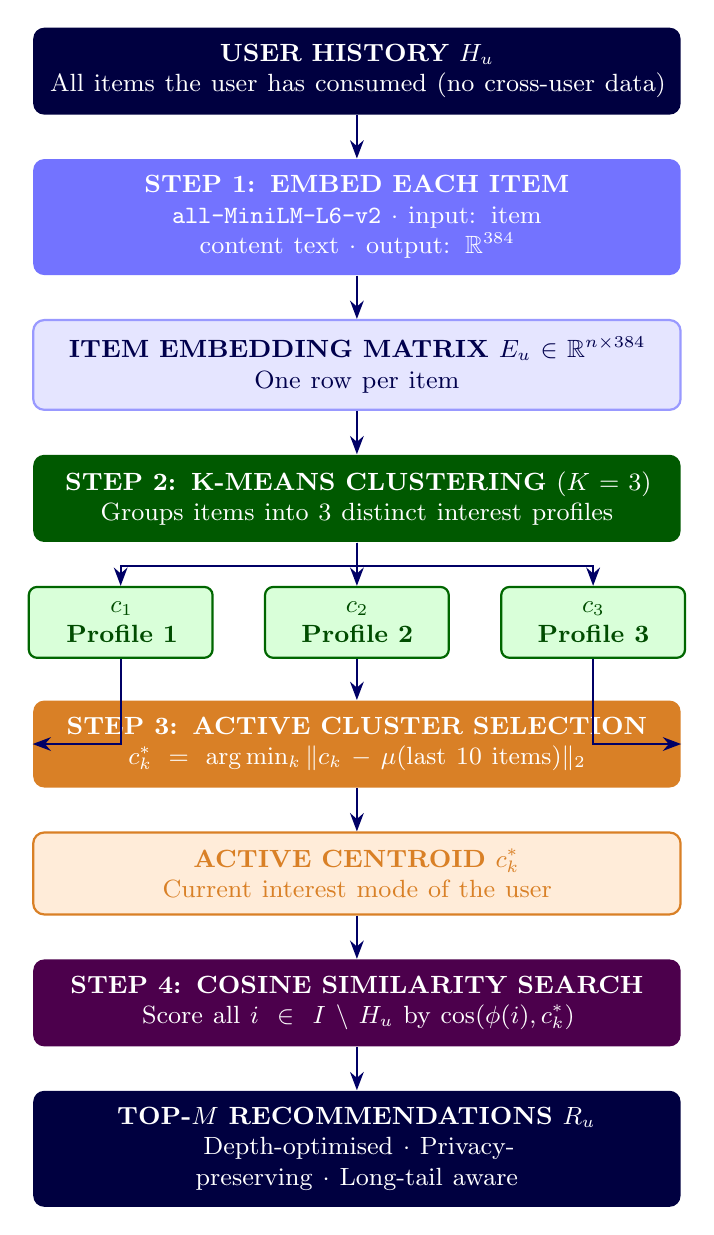
\begin{tikzpicture}[node distance=0.55cm, every node/.style={align=center}]
  \node[navybox]  (hist)   {USER HISTORY $H_u$\\
                             \normalfont\small All items the user has consumed (no cross-user data)};
  \node[bluebox,  below=of hist]  (emb)
        {STEP 1: EMBED EACH ITEM\\
         \normalfont\small \texttt{all-MiniLM-L6-v2} $\cdot$ input: item content text $\cdot$ output: $\mathbb{R}^{384}$};
  \node[lightbox, below=of emb]   (mat)
        {ITEM EMBEDDING MATRIX $E_u \in \mathbb{R}^{n \times 384}$\\ \normalfont\small One row per item};
  \node[greenbox, below=of mat]   (km)
        {STEP 2: K-MEANS CLUSTERING $(K=3)$\\ \normalfont\small Groups items into 3 distinct interest profiles};
  \node[clusterbox, below=of km, xshift=-3.0cm] (c1) {$c_1$\\Profile 1};
  \node[clusterbox, below=of km]                (c2) {$c_2$\\Profile 2};
  \node[clusterbox, below=of km, xshift=+3.0cm] (c3) {$c_3$\\Profile 3};
  \node[brownbox, below=2.0cm of km] (active)
        {STEP 3: ACTIVE CLUSTER SELECTION\\
         \normalfont\small $c_k^* = \arg\min_k \|c_k - \mu(\text{last 10 items})\|_2$};
  \node[warmbox,  below=of active] (ck)
        {ACTIVE CENTROID $c_k^*$\\ \normalfont\small Current interest mode of the user};
  \node[purplebox, below=of ck]   (ann)
        {STEP 4: COSINE SIMILARITY SEARCH\\ \normalfont\small Score all $i \in I \setminus H_u$ by $\cos(\phi(i), c_k^*)$};
  \node[navybox,  below=of ann]   (out)
        {TOP-$M$ RECOMMENDATIONS $R_u$\\
         \normalfont\small Depth-optimised $\cdot$ Privacy-preserving $\cdot$ Long-tail aware};
  \draw[arrow] (hist)   -- (emb);
  \draw[arrow] (emb)    -- (mat);
  \draw[arrow] (mat)    -- (km);
  \draw[arrow] (km.south) -- ++(0,-0.3) -| (c1.north);
  \draw[arrow] (km.south) -- ++(0,-0.3) -| (c2.north);
  \draw[arrow] (km.south) -- ++(0,-0.3) -| (c3.north);
  \draw[arrow] (c1.south) |- (active.west);
  \draw[arrow] (c2.south) -- (active.north);
  \draw[arrow] (c3.south) |- (active.east);
  \draw[arrow] (active) -- (ck);
  \draw[arrow] (ck)     -- (ann);
  \draw[arrow] (ann)    -- (out);
\end{tikzpicture}
\caption{Essence recommendation pipeline. No cross-user data is consulted at any stage.}
\label{fig:pipeline}
\end{figure}

\section{Architectural Comparison}
\label{app:comparison}

\begin{table}[H]
\centering
\caption{Architectural comparison: Essence vs.\ prior systems. The primary distinction is not the clustering mechanism, it is the data requirement and what each system is optimised to find. All four systems are empirically evaluated in this work (Section~\ref{sec:results}), which reports the domain-dependent long-tail recovery result in full.}
\label{tab:comparison}
\small
\begin{tabular}{lcccc}
\toprule
\textbf{Property} & \textbf{CF} & \textbf{MIND} & \textbf{ComiRec} & \textbf{Essence} \\
\midrule
Cross-user data required & Yes & Yes & Yes & \textbf{No} \\
Multiple interest profiles & No & Yes & Yes & \textbf{Yes} \\
Model training required & Yes & Yes & Yes & \textbf{No} \\
Explicit long-tail objective & No & No & No & \textbf{Yes} \\
Embedding source & Co-occurrence & Co-occurrence & Co-occurrence & \textbf{Item metadata} \\
\bottomrule
\end{tabular}
\end{table}

\section{Systems Compared: Full Descriptions}
\label{app:systems}

\textbf{Random.} Recommends $M$ items drawn uniformly from the unseen candidate pool; establishes the floor against which all other systems are compared.

\textbf{Popularity.} Recommends the $M$ globally most-interacted-with unseen items. Non-personalized; included for comparison but not treated as collaborative filtering.

\textbf{CF (ItemKNN).} Item-based $k$-nearest-neighbors collaborative filtering via cosine similarity over the sparse user-item interaction matrix.

\textbf{Content (Average Embedding).} Mean of all the user's item embeddings, retrieving the $M$ most similar unseen items. Standard content-based filtering without interest decomposition.

\textbf{Essence ($K=3$).} Clusters user history into $K=3$ centroids, selects the active centroid by Eq.~\ref{eq:active}, retrieves top-$M$ unseen items by Eq.~\ref{eq:reco}.

\textbf{Last-Item.} Recommends the $M$ unseen items most similar, by cosine similarity, to the single most recent item in the user's training history. The simplest possible recency-based retrieval: no averaging, no decay, no clustering.

\textbf{Avg-Last-10.} Recommends the $M$ unseen items most similar to the uniform mean embedding of the user's last 10 training interactions.

\textbf{Recency-Weighted.} Recommends the $M$ unseen items most similar to an exponentially-decay-weighted mean of the user's last 10 training interactions (decay $=0.9$; the most recent item receives weight $\propto 0.9^{0}$, the tenth-most-recent $\propto 0.9^{9}$, renormalized to sum to 1).

\textbf{MIND.} A hand-implemented dynamic-routing multi-interest network, following Li et al.'s original architecture~\cite{li2019} ($K=4$ interest capsules, a bilinear routing matrix shared across capsules, 3 routing iterations, routing logits initialized $b \sim \mathcal{N}(0, 0.01^2)$). An initial implementation zero-initialized $b$, which --- because the shared bilinear matrix makes the pre-routing representation identical across capsules --- guaranteed every capsule updated identically, silently collapsing the model's effective interest count to 1 regardless of the nominal $K$; caught by a synthetic conformance test and fixed before any number reported in this paper was generated.

\textbf{ComiRec (SA).} A hand-implemented self-attentive multi-interest network, following Cen et al.'s original architecture~\cite{cen2020} ($K=4$ interest capsules, per-capsule learned query projections implemented as a single $K$-output linear layer, softmax attention over sequence positions).

\section{Active Cluster Selection Ablation}
\label{app:ablation}

We test the recency-based active-cluster-selection mechanism (Section~\ref{sec:framework}) against an alternative: selecting the active centroid using the mean embedding of the user's entire training history rather than the most recent $r=10$ interactions.

\begin{table}[H]
\centering
\caption{Active cluster selection ablation, Last.fm-1K (chronological split, $M=10$).}
\label{tab:ablation}
\small
\begin{tabular}{lccc}
\toprule
\textbf{Variant} & \textbf{Recall@10} & \textbf{LT-Recall@10} & \textbf{LT / Content} \\
\midrule
Essence (recency, $r=10$) & 0.0119 & 0.0059 & $2.01\times$ \\
Essence (mean-select, full history) & 0.0035 & 0.0005 & $0.16\times$ \\
Content (Avg Embedding, reference) & 0.0038 & 0.0029 & $1.0\times$ \\
\bottomrule
\end{tabular}
\end{table}

Mean-select performs below even the Content baseline on long-tail recall, consistent with the mechanism collapsing toward Content: selecting the centroid nearest a user's global mean embedding is functionally similar to querying with that mean directly, while incurring the additional cost of clustering without a corresponding benefit. This result is on Last.fm-1K only; we have not verified whether it generalizes to Amazon Books or MovieLens-25M.

\section{Effect of User-Authored Review Embeddings (Amazon Books)}
\label{app:pass2}

As a secondary experiment, we tested whether building user taste profiles from review text (first-person language describing a user's reaction to consumed items) rather than item metadata changes Essence's relative performance.

\begin{table}[H]
\centering
\caption{Amazon Books: metadata embeddings (Pass 1) vs.\ user-review embeddings (Pass 2). Pass 2 builds taste profiles from the user's own review text; candidates are scored using metadata embeddings.}
\label{tab:amazon_pass2}
\small
\begin{tabular}{llccc}
\toprule
\textbf{Pass} & \textbf{System} & \textbf{Recall@10} & \textbf{LT-Recall@10} & \textbf{LT / Content} \\
\midrule
\multirow{3}{*}{Pass 1 (metadata)}
  & CF (ItemKNN) & 0.0031 & 0.0137 & --- \\
  & Content (Avg) & 0.0173 & 0.0124 & $1.0\times$ \\
  & Essence ($K=3$) & 0.0221 & 0.0197 & $1.59\times$ \\
\midrule
\multirow{3}{*}{Pass 2 (user review)}
  & CF (ItemKNN) & 0.0031 & 0.0137 & --- \\
  & Content (Avg) & 0.0027 & 0.0012 & $1.0\times$ \\
  & Essence ($K=3$) & 0.0041 & 0.0034 & $2.83\times$ \\
\bottomrule
\end{tabular}
\end{table}

Absolute recall degrades substantially in Pass 2. Two factors likely contribute: an input-distribution mismatch (taste profiles are built from review-text embeddings while candidates are still scored using metadata embeddings, and although both come from the same encoder, review text and item metadata occupy different regions of the shared embedding space), and review text being a noisier input than structured metadata (a review may describe shipping conditions or personal circumstances unrelated to the item's content). Essence's relative advantage over Content persists in Pass 2 ($2.83\times$ vs.\ $1.59\times$ in Pass 1, both above parity), suggesting the $K$-means clustering mechanism extracts usable interest structure even under degraded input quality. The absolute recall values in Pass 2 are low enough that this comparison carries limited statistical weight; we treat it as a directional observation motivating embedding-input-curation as future work.

\section{Full Statistical-Family Reasoning}
\label{app:fdr}

The Last.fm-1K/Amazon Books baseline comparison (Essence vs.\ each of the nine other systems, per dataset, per metric; 36 comparisons) and the multimodality-stratification test (Essence vs.\ Recency-Weighted, stratified by each user's own per-history silhouette score into low/medium/high clustering-quality tertiles, per dataset, per metric; 18 comparisons) are corrected together as a single 54-comparison Benjamini--Hochberg family, since pooling them changes no comparison's significance verdict relative to correcting them separately (verified directly: recomputing a single pooled BH-FDR correction across all 54 raw $p$-values and comparing every resulting verdict against the two-family version yields zero changes). The MovieLens-25M baseline comparison (18 comparisons) is corrected separately: it was added to this evaluation after the 36 above, but tests the same underlying question, and pooling it was not separately tested. The decile-level cold-start analysis (Essence, and separately each recency-only baseline, vs.\ CF-ItemKNN, restricted to the rarest-item deciles) is corrected as its own family: it asks a narrower, mechanistically distinct question, isolating a single structural property of CF (zero co-occurrence signal for zero-training-interaction items) rather than asking about aggregate performance, and was decided as a separate question before being run --- not a post-hoc re-slicing of the primary comparison chosen because a pooled result was inconvenient.

\section{Extended Discussion}
\label{app:discussion}

\textbf{Mechanism.} Item-based CF records zero long-tail recall on the sparsest dataset, Last.fm-1K, under deterministic ranking; on the denser Amazon Books it surfaces some low-interaction items but pays a large cost to overall recall ($0.0031$, near the bottom of the field). MovieLens-25M is the case where the self-reinforcing popularity loop runs at full strength in the other direction: CF's Recall@10 ($0.0850$) is the highest value recorded anywhere in this study, and Popularity itself ranks 3rd of 10 overall ($0.0517$), yet CF's LT-Recall@10 ($0.0037$) remains far below its own overall Recall@10.

\textbf{Deployment and privacy.} The absolute recall values reported here (roughly $0.005$--$0.03$ under full-catalog evaluation) should be read in light of deployment context: Essence is not proposed as a replacement for a primary, CF-driven feed. On Amazon Books and Last.fm-1K it is better understood as a specialized retrieval path for a dedicated discovery surface (e.g.\ a ``more like this'' interface) where the goal is surfacing items dissimilar from what population-level signals would recommend; this framing does not hold on MovieLens-25M. Separately, because Essence consults no cross-user data at any stage, it remains deployable in settings where CF is not viable at all --- privacy-regulated environments, on-device recommendation without server-side interaction logs, federated settings, and cold-start contexts where no population-level interaction graph exists yet --- a direct architectural consequence, independent of whether Essence wins on a given domain's aggregate metrics.

\section{Extended Limitations and Future Work}
\label{app:limitations}

\textbf{Filter bubble risk.} Peer-isolation removes the serendipity cross-user signals can provide; whether repeated centroid queries cause semantic narrowing is an open empirical question. \textbf{Embedding input curation.} Appendix~\ref{app:pass2} shows noisy embedding inputs degrade performance; the quality of what enters the embedding determines the quality of what Essence can find, and automated curation of embedding input text is a direct practical extension. \textbf{Audio-based embeddings.} Current embeddings derive from item metadata text only; for music, incorporating audio-based representations (sonic texture, timbre, rhythm, harmonic structure) would more precisely model the latent acoustic fingerprint underlying individual taste, and is the primary planned extension of Essence. \textbf{Cross-space embedding alignment.} Appendix~\ref{app:pass2}'s results suggest that aligning review-text and metadata input distributions within the shared embedding space (via contrastive training or a learned projection layer) could unlock the full signal of user-authored representations while maintaining retrieval coherence. \textbf{Active cluster selection.} The recency-based heuristic is simple by design; a learned selection mechanism could improve session-aware accuracy without requiring cross-user training.

\newpage
\section*{NeurIPS Paper Checklist}

\begin{enumerate}

\item {\bf Claims}
    \item[] Question: Do the main claims made in the abstract and introduction accurately reflect the paper's contributions and scope?
    \item[] Answer: \answerYes{}
    \item[] Justification: The abstract and introduction state the domain-dependent, mixed result directly (the Amazon Books win, the Last.fm-1K loss to simple recency retrieval, the MovieLens-25M loss, and the clustering-mechanism null result from the stratification test) rather than only the favorable case; the body (Sections~\ref{sec:results}--\ref{sec:limitations}) matches this framing throughout.

\item {\bf Limitations}
    \item[] Question: Does the paper discuss the limitations of the work performed by the authors?
    \item[] Answer: \answerYes{}
    \item[] Justification: Section~\ref{sec:limitations-findings} and Section~\ref{sec:limitations} discuss scale, $K$-sensitivity, the untested generalization of the ablation and $K$-sensitivity results to MovieLens-25M, the hand-implemented (not pre-trained) status of MIND/ComiRec, and the post-hoc nature of the domain-dependence characterization; Appendix~\ref{app:limitations} extends this further.

\item {\bf Theory assumptions and proofs}
    \item[] Question: For each theoretical result, does the paper provide the full set of assumptions and a complete (and correct) proof?
    \item[] Answer: \answerNA{}
    \item[] Justification: This is an empirical paper; it contains no theorems or proofs.

\item {\bf Experimental result reproducibility}
    \item[] Question: Does the paper fully disclose all the information needed to reproduce the main experimental results?
    \item[] Answer: \answerYes{}
    \item[] Justification: Section~\ref{sec:setup} and Appendix~\ref{app:systems} specify all datasets, splits (chronological, 80/20 per user, seed 42), hyperparameters ($K=3$, $r=10$, decay $=0.9$, $M=10$), the embedding model, and every baseline's exact query construction; Appendix~\ref{app:fdr} specifies the significance-testing methodology in full.

\item {\bf Open access to data and code}
    \item[] Question: Does the paper provide open access to the data and code, with sufficient instructions to faithfully reproduce the main experimental results?
    \item[] Answer: \answerYes{}
    \item[] Justification: Anonymized code and data are available at \url{https://anonymous.4open.science/r/essence-5B7B/README.md}, including full reproduction instructions for every analysis reported in this paper. The repository will be de-anonymized and linked to its permanent location upon deanonymization.

\item {\bf Experimental setting/details}
    \item[] Question: Does the paper specify all the training and test details necessary to understand the results?
    \item[] Answer: \answerYes{}
    \item[] Justification: See Section~\ref{sec:setup} and Appendix~\ref{app:systems}: chronological train/test split, all baseline query constructions, $K$-means configuration, and MIND/ComiRec architecture hyperparameters are specified.

\item {\bf Experiment statistical significance}
    \item[] Question: Does the paper report error bars suitably and correctly defined or other appropriate information about the statistical significance of the experiments?
    \item[] Answer: \answerYes{}
    \item[] Justification: This is a central contribution of the paper (Section~\ref{sec:stats-methodology}, Appendix~\ref{app:fdr}): every comparison uses a paired bootstrap significance test ($10{,}000$ resamples) with reported mean difference, 95\% CI, and Cohen's $d$; Benjamini--Hochberg FDR correction is applied within pre-specified families; BCa resampling cross-checks every raw-significant result.

\item {\bf Experiments compute resources}
    \item[] Question: For each experiment, does the paper provide sufficient information on the computer resources needed to reproduce the experiments?
    \item[] Answer: \answerNo{}
    \item[] Justification: Compute resource details (hardware type, memory, training/inference wall-clock time) are not reported in this paper. This is a gap; the underlying methods (K-means clustering, cosine similarity retrieval, and two small from-scratch neural baselines) are lightweight and do not require specialized hardware, but exact figures are not included.

\item {\bf Code of ethics}
    \item[] Question: Does the research conducted in the paper conform, in every respect, with the NeurIPS Code of Ethics?
    \item[] Answer: \answerYes{}
    \item[] Justification: This work evaluates recommendation algorithms on standard, publicly available, de-identified interaction datasets (Last.fm-1K, Amazon Reviews, MovieLens-25M); it involves no human-subjects research, no crowdsourcing, and no release of models with elevated misuse risk.

\item {\bf Broader impacts}
    \item[] Question: Does the paper discuss both potential positive societal impacts and negative societal impacts of the work performed?
    \item[] Answer: \answerNo{}
    \item[] Justification: The paper discusses privacy-preserving deployment properties (Section~\ref{sec:discussion}, Appendix~\ref{app:discussion}) but does not include a dedicated broader-impacts analysis of positive and negative societal effects; this is a gap given the page-limited format.

\item {\bf Safeguards}
    \item[] Question: Does the paper describe safeguards for responsible release of data or models with high misuse risk?
    \item[] Answer: \answerNA{}
    \item[] Justification: The paper releases no generative models, scraped image data, or other assets with elevated misuse potential.

\item {\bf Licenses for existing assets}
    \item[] Question: Are the creators or original owners of assets used in the paper properly credited and are license and terms of use explicitly mentioned?
    \item[] Answer: \answerNo{}
    \item[] Justification: All datasets and pre-trained models used (Last.fm-1K, Amazon Reviews 2023, MovieLens-25M, \texttt{all-MiniLM-L6-v2}, the TMDb API) are cited to their originating papers/sources, but explicit license names and terms of use are not stated in the paper text.

\item {\bf New assets}
    \item[] Question: Are new assets introduced in the paper well documented and is the documentation provided alongside the assets?
    \item[] Answer: \answerNo{}
    \item[] Justification: The from-scratch MIND/ComiRec implementations and processed dataset subsets are new assets, but no code/data release accompanies this anonymized submission (see the Open Access item above); documentation will accompany the code release upon deanonymization.

\item {\bf Crowdsourcing and research with human subjects}
    \item[] Question: For crowdsourcing experiments and research with human subjects, does the paper include the full text of instructions given to participants and details about compensation?
    \item[] Answer: \answerNA{}
    \item[] Justification: This paper involves no crowdsourcing or human-subjects research; all data consists of pre-existing, publicly released interaction logs.

\item {\bf Institutional review board (IRB) approvals or equivalent for research with human subjects}
    \item[] Question: Does the paper describe potential risks incurred by study participants and whether IRB approval was obtained?
    \item[] Answer: \answerNA{}
    \item[] Justification: No human-subjects research was conducted; no IRB review was required.

\item {\bf Declaration of LLM usage}
    \item[] Question: Does the paper describe the usage of LLMs if it is an important, original, or non-standard component of the core methods in this research?
    \item[] Answer: \answerYes{}
    \item[] Justification: No LLM is a component of any method evaluated in this paper --- Essence, the collaborative-filtering and content-based baselines, MIND, ComiRec, and the significance-testing methodology (paired bootstrap, Benjamini--Hochberg FDR, BCa) are all standard, non-LLM techniques. Consistent with this checklist item's own exemption for ``writing, editing, or formatting,'' AI assistance was used as a development and verification tool during implementation --- including catching a symmetry-breaking initialization bug in our own MIND implementation (Section 4) and flagging several numeric and framing inconsistencies during manuscript preparation, each independently reviewed and confirmed against source data by the authors before being reported. No experimental result, statistical test, or claim in this paper was generated or accepted without direct author verification.

\end{enumerate}

\end{document}
